\chapter{Lipids: More Than Oil and Body Fat}

\begin{kaichang}
Make a small observation. Pour half a cup of clean water, add a spoonful of cooking oil, and stir vigorously with chopsticks for thirty seconds. As you stir, the oil breaks into countless golden droplets tumbling through the water, seemingly about to ``dissolve.'' But stop, and within a minute the droplets find their companions again, merging into a complete layer floating on the water, sharply separated as though the stirring had never happened.

Now consider two other kitchen phenomena. In winter, a bowl of lard is a milky-white solid that takes effort to scoop; the bottle of rapeseed oil beside it remains clear and flowing. Both are ``fats,'' so why does one solidify while the other flows? And egg yolk: cooks know it can ``matchmake'' oil and water into mayonnaise that stays together however long you stir. How does it accomplish what oil and water cannot do alone?

One last question concerns your own body fat: is it the same kind of stuff as the cooking oil in a pan? Beyond ``making you fat,'' what work does it do for which you have never thanked it?

By the chapter's end, these questions will form a complete causal chain. First, write down your guess about oil and water separating.
\end{kaichang}

\section{Visible Fat: Insoluble, Floating, and Solidifying}

\textbf{Translator safety note:} Never create an oil fire for observation. For a small contained pan fire, an adult may slide a lid over it and turn off the heat only if safe, leaving it covered until cool; never use water or move the burning pan. If unsure, leave and call emergency services. See \href{https://www.usfa.fema.gov/prevention/home-fires/prevent-fires/cooking/}{USFA cooking-fire guidance}.

First establish what can be observed, then explain it.

You have seen for yourself that oil and water do not mix. Oil floats rather than sinks, showing that its density is slightly lower, about nine-tenths that of water. It feels slippery and greasy and evaporates slowly: a cup of water dries out in a few days, while a cup of oil scarcely diminishes. Oil burns: overheated oil can catch fire in a pan, so \textbf{never pour water onto an oil fire} (water sinks beneath the oil and vaporizes violently, scattering burning droplets). The correct action is to cover the pan with its lid to cut off air.

Now consider solidification. Lard and butter are soft solids near room temperature, while peanut and rapeseed oils are liquids. All become liquid on heating and return to their respective states on cooling. Thus ``solid or liquid'' is not a fundamental difference between oils and fats, but a matter of which side of room temperature their melting points lie. Remember the terminology: chemistry calls the room-temperature liquids ``oils'' and the solids ``fats,'' but both belong to the same broad family---\textbf{lipids}.

Another easily overlooked phenomenon: milk is uniformly white and never fully ``splits into oil and water,'' however long it stands (only a little cream rises). Mayonnaise is an even more stable oil--water mixture. So the rule of thumb that ``oil and water always separate'' fails when certain substances are present. Exceptions have long been hiding in the kitchen; you simply had not noticed their significance.

\section{Zooming In: A Tail and a Head}

Why do fats and water get along poorly? Zoom to the molecular level. This family has many members; meet four main characters first.

\textbf{First: fatty acids.} They are the starting point for understanding everything else. A fatty acid molecule has two parts: a long chain of a dozen or more carbons covered with hydrogens, purely carbon and hydrogen, with the same ``temperament'' as gasoline, paraffin, and polyethylene (Chapter 36 explained that hydrocarbon chains reject water and favor oil); and a terminal carboxyl group (\chem{-COOH}, the functional group of Chapter 37), which contains oxygen and can shake hands with water. One molecule drags a ``long oil-loving tail'' behind a ``small water-loving head.'' This one molecule with two temperaments seeds every story in the chapter.

\textbf{Second: triglycerides.} Individual fatty acids are awkward to store. Cells attach the carboxyl groups of three fatty acids to the small molecular framework called glycerol through ester bonds (esterification, already seen in Chapter 40). The resulting large molecule is a triglyceride, the main component of cooking oil, lard, and your body fat. All three carboxyl groups are occupied, leaving \textbf{almost no water-loving head}. It is a three-tailed octopus, thoroughly ``unsociable.'' This is oil's true identity.

\textbf{Third: phospholipids.} Replace one fatty-acid tail of a triglyceride with a large water-loving head containing phosphate, and you obtain a phospholipid. Its contrast is stronger than a fatty acid's: two stout oil-loving tails with one large, forceful head. Egg-yolk lecithin and every cell's membrane contain it. Phospholipids specialize in ``bringing oil and water together''---the secret of mayonnaise.

\textbf{Fourth: cholesterol.} Unlike the first three, it has no long tail. Its main body is a stiff ``little board'' of four joined carbon rings, bearing just one small hydroxyl (\chem{-OH}). It fills gaps in cell membranes and provides raw material for many hormones: a bad reputation, but important uses. We will devote a section to it later.

Four characters, three temperaments: purely oil-loving (triglycerides), head-and-tail (fatty acids and phospholipids), and a little board (cholesterol). Remember this classification; their temperaments lead to all the rules that follow.

\section{Tail Shapes: Saturated, Unsaturated, and Trans}

Now answer the second opening question: why is lard solid and rapeseed oil liquid?

The difference is not their origin as ``animal fat or vegetable oil,'' but the \textbf{shape} of their fatty-acid tails. Chapter 36 gave two rules for carbon-skeleton joints: single bonds can rotate freely; double bonds cannot. A chain containing only single bonds can extend straight and is called a \textbf{saturated} fatty acid: its carbons carry all the hydrogens they can, hence ``saturated.'' A carbon--carbon double bond in the middle acts like a welded joint, fixing a bend in the chain; this is an \textbf{unsaturated} fatty acid.

Shape determines packing, which determines melting point. Straight tails stack neatly like chopsticks, bringing molecules close with large contact areas. The intermolecular forces of Chapter 22 add up substantially, requiring a higher temperature to shake them apart. Thus saturated fatty acids, predominant in animal fat, have high melting points and are solid at room temperature. Bent tails pack poorly, like a basket of crooked straws, loosely arranged and falling apart with little warming. Unsaturated fatty acids, predominant in vegetable oils, have low melting points and are liquid at room temperature. Ultimately, ``oil or fat'' is a question of \textbf{whether the tails bend}.

One further detail matters. A double bond can lock the two chain sections on the same side (cis) or opposite sides (trans). Nearly all double bonds in natural vegetable oils are cis and strongly bent. During industrial partial hydrogenation---adding hydrogen at double bonds to thicken oil and improve storage for margarine and shortening---some double bonds remain but are ``straightened'' into trans arrangements. Straighter molecules give higher melting points, better texture, and longer shelf life, but behave worse in your body than cis forms. Large population studies associate trans-fat intake with increased cardiovascular risk and reveal no apparent benefit, so many countries have restricted or prohibited industrial trans fats. Notice the evidential wording: ``associated with increased risk,'' not ``one bite poisons you.'' Dose always matters; occasional exposure differs from sustained high intake. ``Hydrogenated vegetable oil,'' ``margarine,'' and ``shortening'' on ingredient lists offer clues to older processing, but formulations are improving, so consult nutrition labels for actual amounts.

\begin{qiaoliang}
Why can a double bond lower melting point by dozens of degrees? Count contacts. Model fatty-acid tails as rows of beads: two straight 18-carbon chains lying together offer a dozen or more bead-to-bead contact points, each contributing a weak intermolecular attraction. Put a cis bend in the middle, and the chains resemble misaligned zippers, perhaps retaining fewer than half those contacts. Each attraction is small, but melting point reflects their \textbf{sum} opposing thermal motion. Halve the sum, and the required ``shaking temperature'' drops sharply: straight, 18-carbon stearic acid melts around $69\,^{\circ}\mathrm{C}$; oleic acid, also 18-carbon but with one cis double bond, melts around $13\,^{\circ}\mathrm{C}$. One double bond, more than fifty degrees---an exceptionally direct demonstration of ``structure determines properties.''
\end{qiaoliang}

\section{Oil Does Not Fear Water; Water Loves Itself}

Here is the chapter's most important rule. Calling oil ``hydrophobic'' makes it sound as though oil molecules dislike and avoid water molecules. Wrong. Molecules have no likes or dislikes, and weak attractions actually exist between oil and water. The real protagonist is \textbf{water's interaction with itself}.

Recall Chapters 21 and 22: water molecules pull on one another through hydrogen bonds, forming a vast network continually breaking and reforming. This network is energetically favorable; each water molecule tries to hold as many neighbors' ``hands'' as possible. Now an oil molecule enters. Uncharged and unable to hydrogen-bond, it resembles a stone intruding at a dance. Surrounding waters cannot grasp it, so they cling to one another, arranging a more ordered ``cage'' around its surface and forfeiting hydrogen-bond partners with whom they could otherwise freely combine. Statistically, in Chapter 28's language, this ``cage water'' has fewer possible arrangements and lower entropy---a poor deal.

What can the system do? There is a remarkably simple way out: \textbf{push the oil molecules together}. A thousand dispersed oil molecules require a thousand little cages. Cluster them into one large oil droplet, and a cage need cover only its surface, constraining fewer water molecules and freeing many more---total entropy rises. The droplets scattered by your stirring reunite not because they are ``homesick,'' but because the water molecules' collective statistical account squeezes them back together. This is the \textbf{hydrophobic effect}: no new force between oil and water, but the water hydrogen-bond network ``outsourcing'' its unwelcome guests to minimize its losses.

Now phospholipids take the stage. With one water-loving head but two tails, they can neither dissolve completely nor settle for being squeezed entirely into an oil droplet. Their compromise is beautiful: heads in the water, tails hidden inside, thousands or tens of thousands automatically arranging into \textbf{two layers}, heads outward toward water and tails together between the layers. No blueprint or supervisor is needed. Scatter phospholipids into water, and they assemble into bilayers, even curving into closed little spheres enclosing a small parcel of water.

\begin{center}
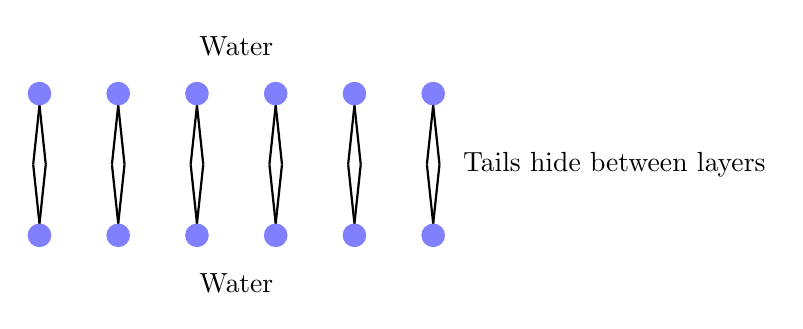
\begin{tikzpicture}[scale=1]
\foreach \x in {0,1,2,3,4,5} {
  \fill[blue!50] (\x,2.0) circle (0.15);
  \draw[thick] (\x,1.85) -- (\x-0.08,1.1);
  \draw[thick] (\x,1.85) -- (\x+0.08,1.1);
  \fill[blue!50] (\x,0.2) circle (0.15);
  \draw[thick] (\x,0.35) -- (\x-0.08,1.1);
  \draw[thick] (\x,0.35) -- (\x+0.08,1.1);
}
\node at (2.5,2.6) {Water};
\node at (2.5,-0.4) {Water};
\node at (7.3,1.1) {Tails hide between layers};
\end{tikzpicture}
\end{center}

The circles are water-loving heads and the short lines oil-loving tails---a human-made representation. Real phospholipids do not have such round heads or straight tails. A two-layer phospholipid ``membrane'' is only about 5 nanometers thick, yet forms every cell's outer wall. Its construction is astonishing: \textbf{no builder, just the statistical rule of the hydrophobic effect}. The full membrane story---controlling traffic and generating voltage---belongs to Chapter 51. For now, simply recognize that boundaries can grow by themselves.

\textbf{Translator safety note:} The egg-yolk mixture below is an experiment, not edible mayonnaise. Keep raw egg and experimental utensils away from ready-to-eat food, and wash hands and surfaces. Edible uncooked egg recipes require appropriate pasteurized ingredients; see \href{https://www.fda.gov/food/retail-food-industryregulatory-assistance-training/assuring-safety-eggs-and-menu-and-deli-items-made-raw-shell-eggs}{FDA egg-safety guidance}.

\begin{shiyan}
\textbf{Let Oil and Water Shake Hands: Emulsification}

Materials: three identical small clear bottles with lids, cooking oil, water, a raw egg yolk, a drop of dishwashing detergent, and a toothpick.

Steps:
\begin{enumerate}[itemsep=1pt]
\item Fill each bottle about one-third with water, then add a spoonful of cooking oil.
\item Add nothing else to bottle 1. Close tightly, shake for 20 seconds, then leave it standing and time the separation.
\item Use the toothpick to add a little yolk to bottle 2. Again shake for 20 seconds, then let it stand and observe.
\item Add a drop of detergent to bottle 3, shake for 20 seconds, and observe it standing.
\end{enumerate}

What to observe: does bottle 1 develop a sharp boundary within a minute? Does bottle 2 become cloudy yellow and thick, staying mixed for a long time? How long do bottle 3's foam and cloudiness last? Think about egg-yolk lecithin and detergent molecules at the oil--water interface: which way do their heads and tails point?

Safety note: these household materials make this a reassuringly simple activity, but \textbf{do not eat any materials used in it}. Raw eggs may carry bacteria, so wash your hands afterward. Clean the bottles before recycling.
\end{shiyan}

\section{Symbols: Registering the Four Characters}

Symbols become meaningful once the concepts are clear. Let us register the four characters in chemical notation.

Stearic acid, a straight, saturated 18-carbon fatty acid:
\[\chem{CH_3(CH_2)_{16}COOH}\]
There are 17 chain carbons and one in the carboxyl, totaling 18. Oleic acid also has 18 carbons, with just one cis double bond in the middle:
\[\chem{CH_3(CH_2)_7CH{=}CH(CH_2)_7COOH}\]
See the pattern? Identical carbon counts, differing by one double bond---one welded bend lowering the melting point by more than fifty degrees.

Triglyceride formation is a triple performance of Chapter 38's condensation reaction: glycerol has three hydroxyls (\chem{-OH}), each joining a fatty-acid carboxyl and expelling one water molecule, making three ester bonds:
\[\chem{C_3H_8O_3} + 3\,\chem{C_{17}H_{35}COOH} \rightarrow \chem{C_{57}H_{110}O_6} + 3\,\chem{H_2O}\]
The product is a typical animal-fat molecule. All three fatty acids here are stearic acid; real fats usually mix tails of different lengths, straight and bent. In reverse, adding water to cut ester bonds is hydrolysis. Your digestive system uses it to dismantle oil, and soap factories use it to make soap (Chapter 40's saponification): the same bond, two ways of breaking it.

Cholesterol's full structural formula is complicated. Remember only its four fused carbon rings---three six-membered and one five-membered---and molecular formula \chem{C_{27}H_{46}O}. Its 27 carbons form an almost entirely hydrocarbon framework with only one oxygen, making it as water-shy as oil, never wandering alone in blood. This property will soon matter greatly.

\section{One Gram of Fat: The Energy Account}

Besides giving you a softer cushion when you sit, what does body fat do? Start with its most famous account: energy storage.

\begin{qiaoliang}
Burn one gram of each: fat releases about \ud{38}{kJ}, carbohydrates only about \ud{17}{kJ}---a difference of more than twofold. Why? The key is ``how much has already burned.'' Combustion is carbon and hydrogen combining with oxygen (Chapter 26). A carbohydrate skeleton is covered with oxygen: glucose, \chem{C_6H_{12}O_6}, has nearly equal numbers of carbon and oxygen atoms. Its carbon is effectively ``half burned already,'' leaving limited energy for further burning. A fatty-acid chain consists almost entirely of carbon--hydrogen bonds, with every carbon still ``fresh, unburned firewood.'' Oxidizing it from end to end naturally releases more.

Storage cost makes the difference greater. Cells store carbohydrate as water-loving glycogen, which binds 2--3 grams of water per gram. Hydrophobic fat stores cleanly as pure energy. Including water's mass, fat's effective energy density can exceed carbohydrate's by sixfold. For an animal migrating, hibernating, or facing hunger, storing carbohydrate means traveling with a water tank; fat is the genuinely lightweight option.
\end{qiaoliang}

Estimate your own order of magnitude. An ordinary adult carries about \ud{10}{kg} of fat, varying greatly with body build. At \ud{38}{kJ} per gram, that is $10\,000 \times 38 \approx \ud{3.8\times 10^{5}}{kJ}$. Daily total expenditure is about \ud{8000}{kJ}. Divide, and this reserve could theoretically last more than forty days. Whole-body glycogen totals only a few hundred grams, not even one day's supply. Migratory birds flying thousands of kilometers without eating and camels carrying a dozen or more kilograms of fat---not water---in their humps rely on this account. Fat oxidation also produces water, providing a bonus supply. Of course, this estimate is idealized: real starvation also breaks down protein, with layers of hormonal regulation, so people cannot simply burn through those forty days ``cleanly.'' But the scale explains evolution's choice: long-distance, long-term reserves require fat.

\section{Insulation, Cushioning, and Signals}

Energy storage is only the first page of fat's résumé.

\textbf{Insulation.} Fat conducts heat slowly, providing a close-fitting insulating layer. Seals, whales, and penguins move comfortably through icy water thanks to several centimeters of subcutaneous fat; part of your relative cold sensitivity or resistance also lies in this layer's thickness. Whales' special layer is called blubber, doing double duty as insulation and energy reserve.

\textbf{Cushioning.} Your kidneys and eyeballs do not rest directly against the body wall: soft fat pads support and wrap them, absorbing shocks from walking, jumping, and collisions. Without them, an ordinary fall might injure internal organs.

\textbf{Signals and raw materials.} This easily overlooked entry most strongly overturns the notion of fat as ``dead inventory.'' Cholesterol's little board starts an entire production line: sex hormones (estrogens and testosterone), adrenal cortical hormones, fat-digesting bile acids, and vitamin D synthesized in sun-exposed skin all derive from cholesterol. Without it, the line shuts down. Fat cells themselves are not silent warehouses either: they secrete signaling molecules, such as leptin, to report stocks to the brain and help regulate appetite. In other words, body fat is also an endocrine organ, constantly calling your brain.

\section{How Scientists Know: One Layer or Two?}

\begin{zhengju}
Does a cell membrane contain one phospholipid layer or two? The question seems unanswerable: the membrane is too thin for even the last century's best light microscopes. In 1925, Dutch scientists Evert Gorter and François Grendel found an elegant experimental detour.

They chose red blood cells: mature cells have no nucleus or organelles, leaving almost only the outer membrane, without other membranes interfering. First, extract all lipids from a known number of cells. Second, spread them on water as a film one molecule thick. Third, measure that film's total area and compare it with the red cells' surface area.

The result: the spread film's area was about \textbf{twice} the cells' surface area. A single-layer membrane should give equal areas; twice the area implies two layers, matching today's textbook phospholipid bilayer.

But the story's second half matters equally. Later researchers recalculated and found two offsetting errors: the red-cell surface area had been underestimated (cells are flattened disks, not the smooth spheres assumed), and acetone had not extracted all the lipids. By chance, the errors canceled and the answer was right. Electron microscopes appeared in the 1950s, letting researchers directly ``see'' membrane structure and firmly establish the bilayer. The lesson: a classic experiment can reach the right conclusion through incomplete reasoning. Science is never one experiment's final verdict, but a long process of cross-checking methods and uncovering errors one by one.
\end{zhengju}

\section{Cholesterol's Transport Fleet: Lipoproteins}

Now address the topic most easily distorted in this chapter.

Blood consists mainly of water, while triglycerides and cholesterol avoid it. Traveling these vascular ``canals'' requires ``boats'': \textbf{lipoproteins}, spherical particles carrying triglycerides and cholesterol inside, with an outer single phospholipid layer (heads facing blood) and proteins that also serve as ``delivery-address labels.'' The body builds several boat sizes, ranked from high to low density. Two are most often discussed: low-density lipoprotein (LDL) and high-density lipoprotein (HDL).

Hence the familiar mnemonic: LDL is ``bad cholesterol,'' HDL ``good cholesterol.'' Half right, but importantly half wrong. Its limits need explaining:

\begin{itemize}[itemsep=2pt]
\item \textbf{Neither LDL nor HDL is cholesterol.} They are boats; cholesterol is cargo, identical on both boats. Cholesterol molecules are not intrinsically good or bad: they are essential for membranes and hormones, and the body synthesizes about one gram daily, more than you obtain from food.
\item \textbf{The ``bad'' part is the destination.} Extensive, mutually supporting evidence from population cohorts, genetics, and randomized drug trials shows that persistently excessive LDL particles enter and accumulate beneath arterial endothelium, initiating atherosclerotic plaques. The relationship is clearly causal, not merely correlational. Calling high LDL a risk factor rests on strong evidence.
\item \textbf{The ``good'' half is much less certain than the mnemonic suggests.} HDL returns excess tissue cholesterol to the liver for recycling. Populations with higher HDL have lower cardiovascular risk, earning its ``good'' reputation. Yet correlation is not causation: several drugs designed to raise HDL \textbf{failed to reduce heart attacks and strokes} in large randomized trials. This strongly suggests that HDL level may be more a ``dashboard'' of bodily condition than a directly steerable ``wheel.''
\item \textbf{Risk is a whole picture, not one number.} LDL has size subtypes, and particle count more closely reflects risk than total mass; smoking, blood pressure, glucose, and family history share the same risk assessment. A clinician interprets the two arrows on a test report in your overall context. This chapter explains mechanisms, not individual diagnosis or treatment.
\end{itemize}

In one sentence, ``good and bad cholesterol'' confuses boats with cargo and correlation with causation, flattening multidimensional population risk into a two-number mnemonic. It is acceptable shorthand for science communication, but inadequate as an action guide.

\textbf{Translator safety note:} Cholesterol's essential cellular roles do not mean prescribed LDL lowering is harmful or unnecessary. Do not stop medication or change treatment based on the passage below; appropriate goals depend on clinical risk and professional assessment. See \href{https://www.nhlbi.nih.gov/health/blood-cholesterol/treatment}{NHLBI cholesterol-treatment guidance}.

\begin{wuqu}
``Cholesterol is harmful: eat as little as possible, ideally reduce it to zero.'' Wrong at both ends. First, cholesterol is essential: without it, membrane fluidity fails and sex hormones, vitamin D, and bile acids run out. Even if you eat none, the liver synthesizes about one gram daily. Second, lower blood measurements are not always better: risk comes from \textbf{long-term excessive accumulation} of LDL particles in artery walls, not the mere existence of cholesterol. The real management target is persistent transport-system imbalance, not a molecule essential to life. Another advertising claim deserves dismantling: ``cholesterol-free'' on vegetable-oil bottles is redundant because plants do not synthesize cholesterol, as correct and unnecessary as ``contains no beef'' on mineral water.
\end{wuqu}

\section{Where These Models Fall Short}

Every chapter must define its models' limits. Here are three.

\textbf{First, the hydrophobic effect is not an absolute force.} It is a statistical outcome of water's hydrogen-bond network, with strength varying by temperature (usually increasing on warming). With amphiphilic molecules that like both oil and water, it yields ordered assemblies rather than separation: micelles, bilayers, and vesicles, their particular form depending on head-to-tail size ratios. Imagining an impassable gulf between oil and water misses this entire landscape of self-assembly.

\textbf{Second, ``saturated means solid, unsaturated means liquid'' is simplified.} Natural fats mix dozens of triglycerides, with a softening range rather than one melting point. The same fat can also form several crystal arrangements with different melting points and textures. Chapter 24's bloomed chocolate showed cocoa butter changing formation. Tail straightness is only the first approximation to melting point, not the whole explanation.

\textbf{Third, and most easily overstepped, evidence linking dietary fats and health varies greatly in strength.} ``Trans fats are harmful'' and ``excess LDL promotes atherosclerosis'' have mutually supporting population, genetic, and randomized-trial evidence and are relatively firm conclusions. Claims such as ``this oil fights cancer,'' ``this fatty acid boosts the brain,'' or ``eating fat directly becomes body fat'' often rest only on observational studies or even advertising copy. Observational studies find clues well but inherently struggle to distinguish causation: people favoring an oil might also exercise more, earn more, and see doctors more often. Dose, individual differences, and overall diet can each reverse a conclusion. This chapter offers mechanisms and methods for assessing evidence; leave your personal dietary choices to clinicians and dietitians.

\section{Back to the Cup of Oil and Water}

Now check the opening questions one by one.

Why does oil separate again after stirring? Water's hydrogen-bond network resists making extra cages around oil. Squeezing oil together and minimizing the interface serves the whole network's statistical account, not oil's ``sulking.'' Oil floats simply because its density is slightly lower.

Why is lard solid and rapeseed oil liquid? Count tail double bonds. Lard's fatty-acid tails are mostly straight, packing neatly with enough intermolecular attraction to resist room-temperature motion. Rapeseed oil's tails have cis bends, pack loosely, and are already liquid at room temperature. One family, one bend's difference.

How does egg yolk reconcile oil and water? Lecithin's one head and two tails occupy the interface, head in water and tails in oil, individually ``wrapping and registering'' countless tiny oil droplets so water can no longer squeeze them together. This is emulsification. Before sale, milk is homogenized: its fat globules are broken extremely small and wrapped by proteins and phospholipids, leaving no floating oil patches in your drink.

Your body fat really is the same molecular family as cooking oil---triglycerides. But it is not dead inventory: it is forty days' energy reserve, shock absorbers for kidneys and eyes, close-fitting winter insulation, and an endocrine organ continuously signaling the brain. It can malfunction (persistently excessive stores cause inflammation and metabolic disorders, a medical topic), but it was never a bodily mistake. It is an energy-storage solution refined through billions of years of evolution, one reason all your ancestors survived uncertain food supplies long enough for you to exist.

\section{A Boundary Exists; Who Guards the Gate?}

This chapter built an extraordinary molecule: the phospholipid. Without instructions, the hydrophobic effect alone lets it enclose a ``room'' in water, separating inside from outside. Chapter 45 called a boundary life's first piece of luggage; now you have seen how it packs itself. Chapter 51 will revisit the membrane's selective traffic and voltage maintenance, an entire precision customs system.

But perhaps you see a problem: if an automatically enclosed room has watertight walls, how can its contents eat and remove waste? A pure phospholipid bilayer almost completely blocks water and ions. Real membranes embed devices for opening doors, pumping water, and sending signals, none made of lipids. They belong to the next chapter's protagonist: proteins, molecular machines folded from twenty kinds of parts. Lipids have set the stage; in Chapter 48, the actors arrive.

\begin{tiaozhan}
(Skipping this does not affect the main thread.) The hydrophobic-effect account can be written as $\Delta G = \Delta H - T\Delta S$ (Chapter 28). Around dispersed oil molecules, ordered ``cage water'' has low entropy. When oil clusters, many water molecules regain freedom, making $\Delta S$ positive and $-T\Delta S$ negative, pulling $\Delta G$ negative so the process is spontaneous. Notice a counterintuitive detail: the driving force for ``oil--water separation'' comes mainly from \textbf{entropy}, not energy. The mixture's energy change ($\Delta H$) is small and sometimes even endothermic, yet entropy increase still accomplishes the separation. More intriguingly, the same physical rule has a second full-time job: during protein folding, hydrophobic amino-acid side chains are squeezed inward while water-loving ones remain outside. Chapter 48 will show how this statistical rule writes much of a protein's three-dimensional shape in water.
\end{tiaozhan}

\section*{Exercises}

\begin{sikaoti}
\item Sketch a phospholipid bilayer using circles for water-loving heads and zigzags for oil-loving tails. Mark which sides contact water and note, ``This is a human-made representation.'' Then draw a closed phospholipid vesicle in water and identify its contents.
\item Calculate storage: a hiker needs reserves releasing about $\ud{40000}{kJ}$. How many kilograms must be carried as fat versus glycogen (about $\ud{17}{kJ}$ per gram, with approximately 2 grams of bound water per gram)? Use the result to explain why hibernators store fat rather than carbohydrate.
\item A margarine factory wants to turn liquid vegetable oil into a spreadable room-temperature solid. The chapter suggests two routes: hydrogenate double bonds or ``straighten'' them. What does each change in the molecule, and what price does each pay? (Hint: one loses nutritional advantages; the other produces trans fats.)
\item An older relative says, ``My report shows high `good cholesterol,' so I can stop worrying.'' Write three sentences using the boats-and-cargo analogy to explain what is right and what is unreliable in that statement.
\item Gorter and Grendel found the spread lipid area to be roughly twice the red-cell surface area and inferred a bilayer. If they had measured 1.5 times, could they simply announce ``one and a half layers''? List at least two potential experimental errors and additional measurements to distinguish them.
\item The chapter says oil--water separation is driven ``mainly by entropy, not energy.'' Using Chapter 28's intuition, explain why oil being pushed together into greater order does not violate entropy increase. (Hint: are you counting only oil, or water too?)
\end{sikaoti}
